\subsection{Modelagem 3D das soluções}
Os estudos das possíveis soluções exigiu uma visualização mais detalhada do
volume livre no interior da turbina. Para isso, foi recriado o ambiente da
turbina em CAD 3D no SolidWorks, a partir dos desenhos 2D de seção da turbina
fornecidos pelo cliente.
O modelo tridimensional do aro câmara permite o estudo e o dimensionamento geométrico de
alcance do manipulador para cada solução. Não foram necessários
detalhamentos de todos os componentes, podendo ser apenas considerados, e
representados com maior precisão, os perfis externos do túnel à montante, o
estator, o rotor e uma pequena região à jusante, além dos acessos
por escotilha superior e inferior.
A figura~\ref{fig::ambiente3d} apresenta o ambiente da turbina em CAD e os
possíveis acessos para realização das intervenções.

\begin{figure}[h!]
\centering
	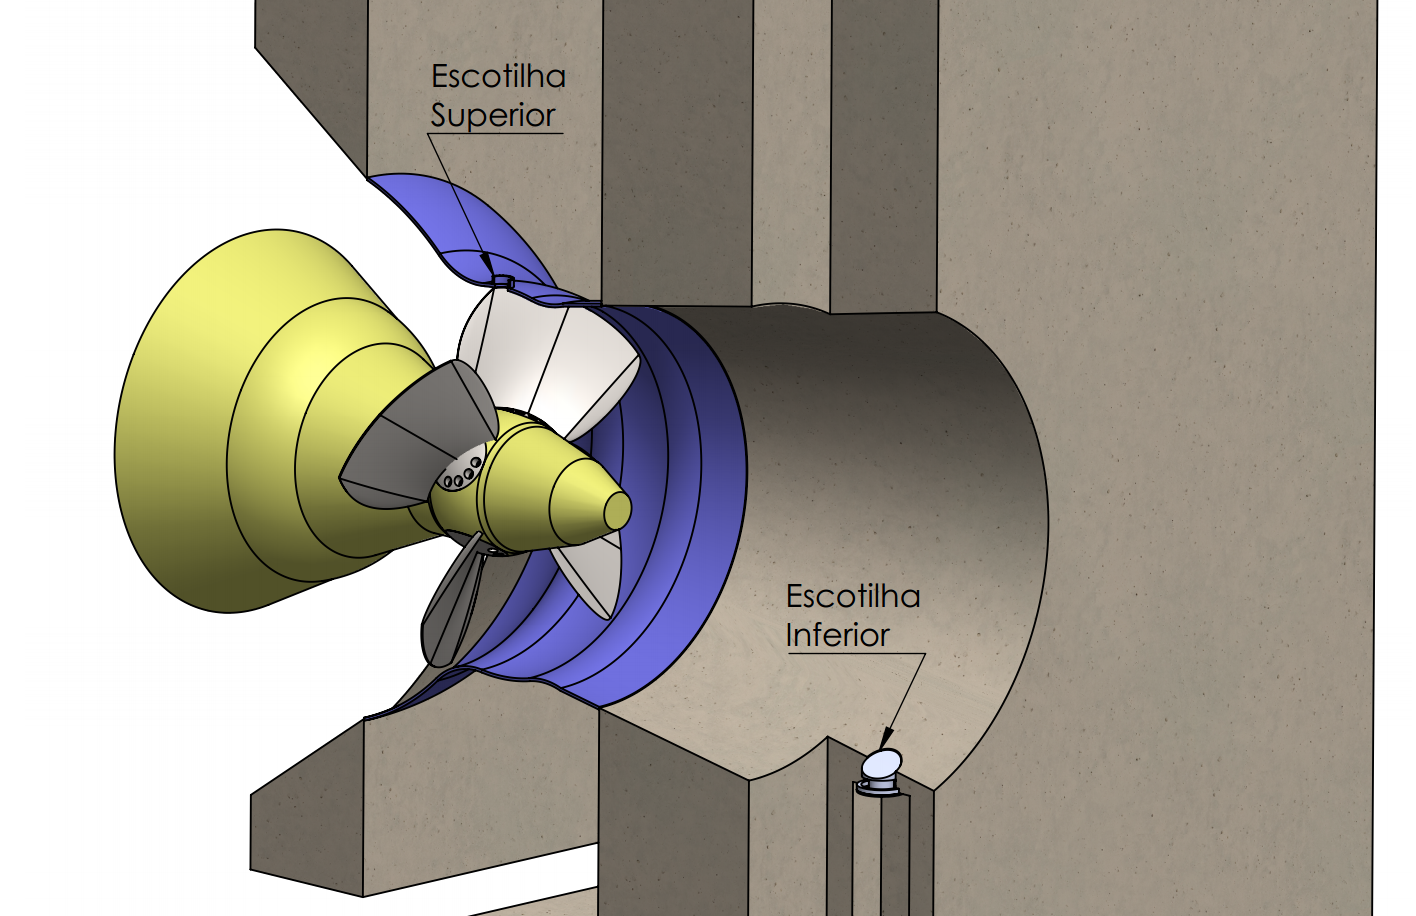
\includegraphics[width=\columnwidth]{figs/estudo/solid/ambiente_3d} 
	\caption{Ambiente 3D da Turbina, em SolidWorks}
	\label{fig::ambiente3d}
\end{figure}

A solução pela escotilha superior, devido ao espaço reduzido de entrada, não
permite a utilização de manipuladores de grande porte, sendo escolhido o KUKA
LBR 820. Este manipulador não possui alcance para realizar a operação em toda a
pá de uma só vez, exigindo uma base customizada que permita o
posicionamento do manipulador para realização das operações por etapas. Para
isso, foi estudada uma estrutura de base que permitisse diferentes
posicionamentos para o manipulador no interior do aro câmara, de forma que este
pudesse cobrir toda a superfície da pá. A base consiste em 3 braços
telescópicos que permitem a extensão do sistema para prover o alcance
necessário ao manipulador e o recolhimento para uma configuração incial que
permita a entrada do manipulador no aro câmara com segurança, sem o risco de
choques ou interferências indesejadas. Além disso, uma junta rotativa oferece mais um grau
de liberdade para o sistema, facilitando o acesso do manipulador à toda ar
superfície da pá. Os atuadores são acionados eletricamente com sensor de
posicionamento. Atuadores de esferas recirculantes foram escolhidos devido à
baixa folga e precisão elevada. A estrutura da base é composta por cilindros de
diâmetro maximizado e pequena espessura, o que oferece um momento de inércia
polar elevado e baixo peso, fornecendo grande rigidez à flexão e minimizando
assim erros de posicionamento e vibração excessiva. A
figura~\ref{fig::base_recolhida} e a figura~\ref{fig::base_extendida} apresentam
o conceito da base do manipulador em duas configurações: recolhida (configuração
de entrada) e extendida (configuração de operação).

\begin{figure}[h!]
\centering
	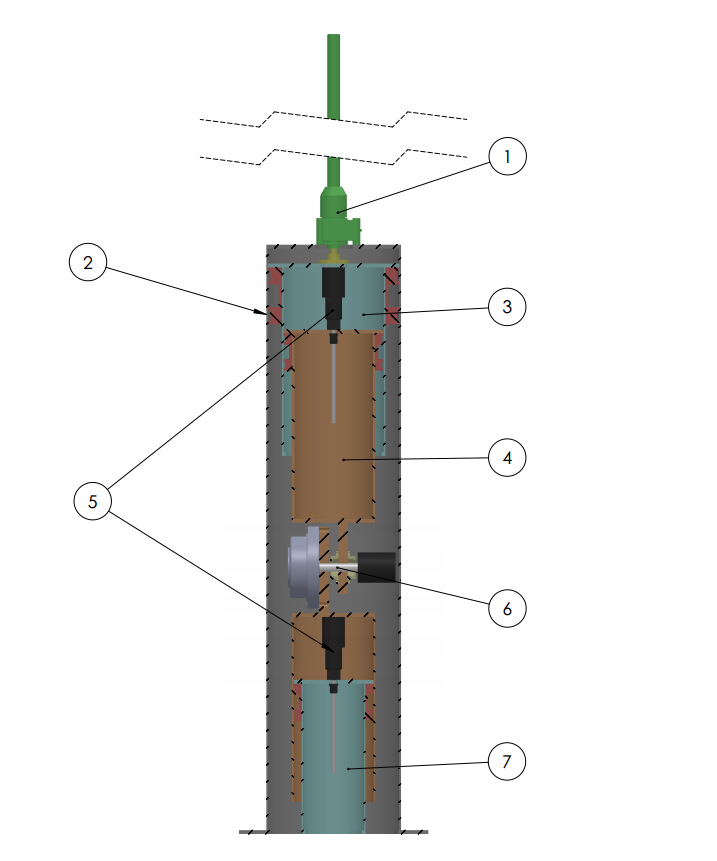
\includegraphics[width=\columnwidth]{figs/estudo/solid/Base_Recolhida.PNG} 
	\caption{Detalhes em corte da base na configuração inicial recolhida}
	\label{fig::base_recolhida}
\end{figure}

\begin{figure}[h!]
\centering
	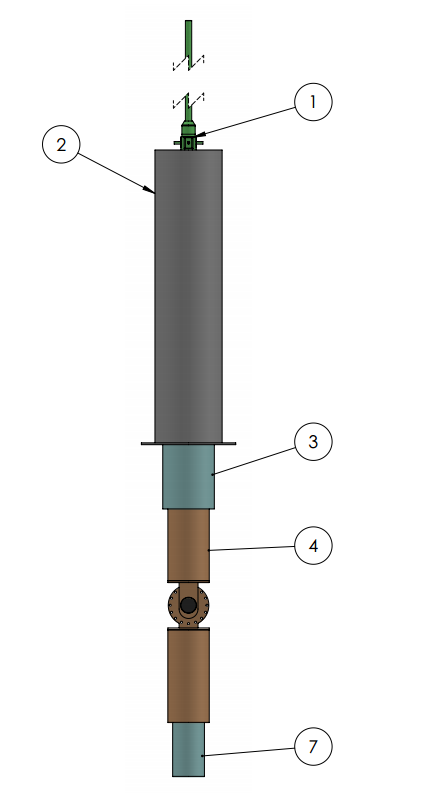
\includegraphics[width=\columnwidth]{figs/estudo/solid/Base_Extendida.PNG} 
	\caption{Base na configuração totalmente extendida}
	\label{fig::base_extendida}
\end{figure}

Os componentes principais da base estão representados nas
figuras~\ref{fig::base_recolhida} e~\ref{fig::base_extendida}, são: 1.atuador
linear por sem-fim coroa; 2.base fixa; 3.braço prismático \#1; 4.braço
prismático \#2; 5.atuadores lineares; 6.junta rotativa; 7.braço prismático \#3.

A figura~\ref{fig::base_ambiente3d_recolhida} demonstra a base com o
manipulador KUKA LBR 820 e as dimensões extremas, em milímetros, estimadas para o
interior e para fora da turbina, na configuração inicial de entrada no aro
câmara pela escotilha superior.
A figura~\ref{fig::base_ambiente3d_extendida} apresenta a base com o manipulador
em uma configuração qualquer de operação, demonstrando o ganho de alcance e
generalidade de posicionamento fornecidos pela base.

\begin{figure}[h!]
\centering
	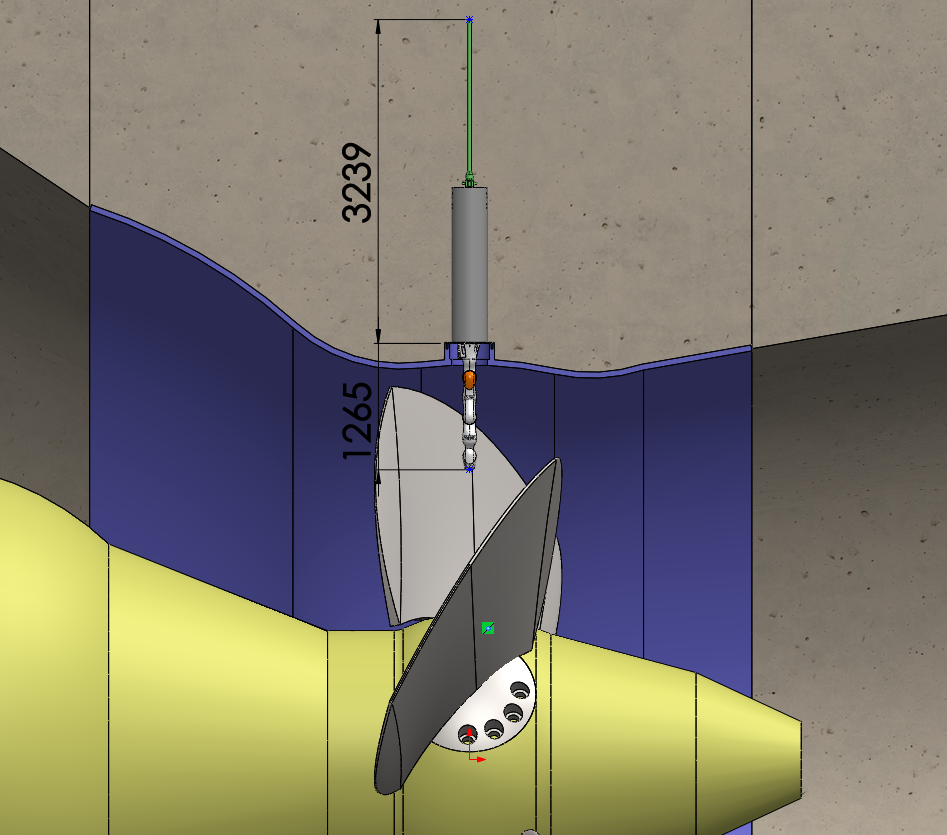
\includegraphics[width=\columnwidth]{figs/estudo/solid/Base_Ambiente3d_Recolhida.png} 
	\caption{Base na configuração inicial no ambiente da turbina}
	\label{fig::base_ambiente3d_recolhida}
\end{figure}

\begin{figure}[h!]
\centering
	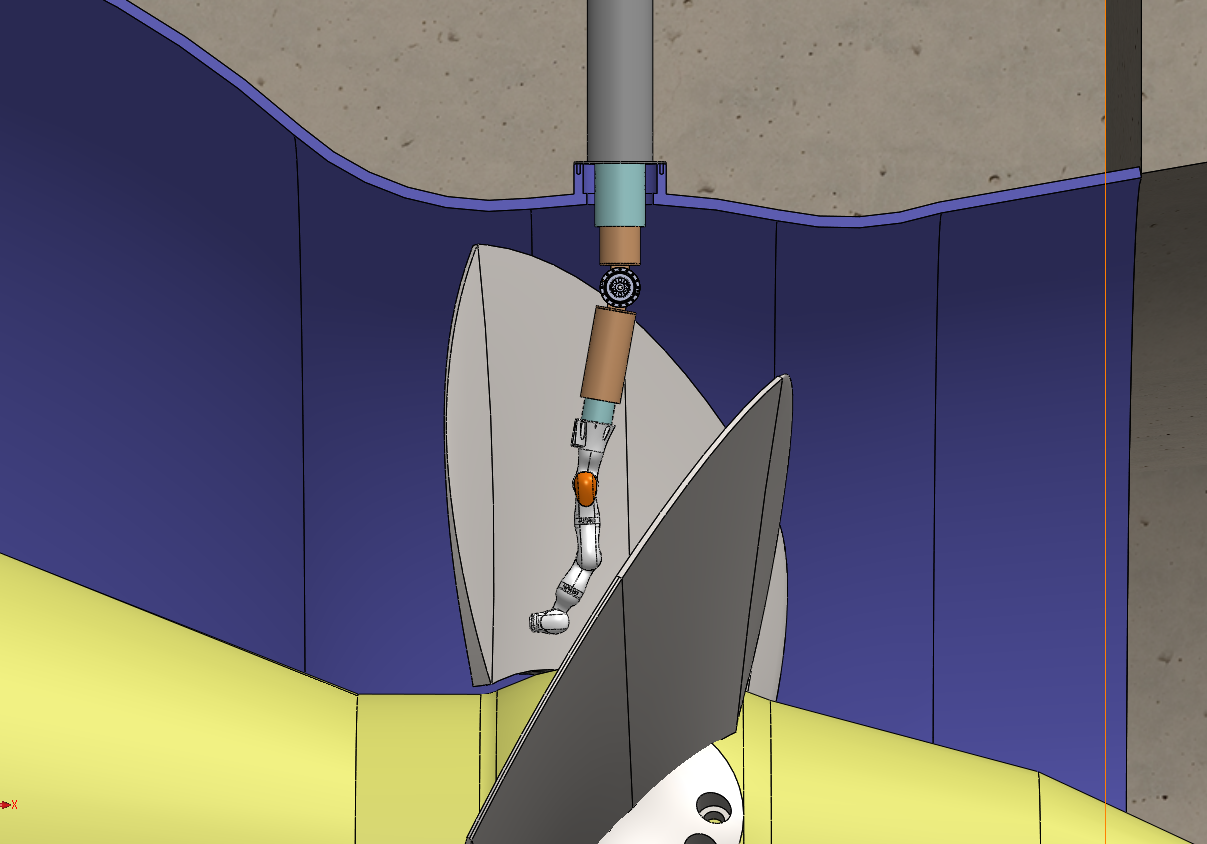
\includegraphics[width=\columnwidth]{figs/estudo/solid/Base_Ambiente3d_Operacao.PNG} 
	\caption{Base em uma geral configuração de operação}
	\label{fig::base_ambiente3d_extendida}
\end{figure}








